\documentclass[11pt, oneside]{article}   	% use "amsart" instead of "article" for AMSLaTeX format
\usepackage{geometry}                		% See geometry.pdf to learn the layout options. There are lots.
\geometry{letterpaper}                   		% ... or a4paper or a5paper or ... 
%\geometry{landscape}                		% Activate for for rotated page geometry
%\usepackage[parfill]{parskip}    		% Activate to begin paragraphs with an empty line rather than an indent
\usepackage{graphicx}				% Use pdf, png, jpg, or eps� with pdflatex; use eps in DVI mode
								% TeX will automatically convert eps --> pdf in pdflatex		
\usepackage{amssymb}
\usepackage{amsmath}

\title{Theorems of Pappus}
%\author{The Author}
\date{}							% Activate to display a given date or no date

\graphicspath{{/Users/telliott_admin/Dropbox/Tex/png/}}

\usepackage{hyperref} 
\begin{document}

\maketitle
%\section{}
% \subsection*{R code}
% \begin{lstlisting}  \end{lstlisting}
% \begin{center} 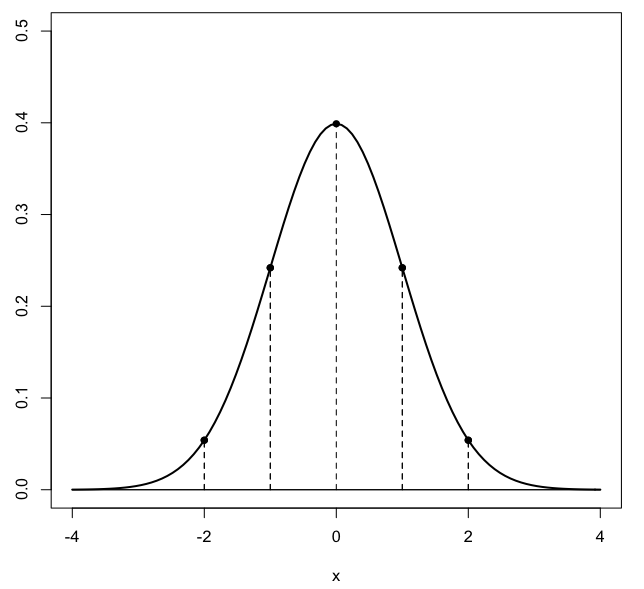
\includegraphics [scale=0.4] {gauss3.png} \end{center}
% \begin{bmatrix} a  &  b \\ c  &  d \end{bmatrix}
% \bigg |_

\large
Pappus' centroid theorem is actually a pair theorems about certain kinds of solids, called solids of revolution, where a curve $C$ is revolved around a central axis.  The two theorems relate to the surface area and volume.  There is a nice article about it at Mathworld
\vspace{2 mm}

\url{http://mathworld.wolfram.com/PappussCentroidTheorem.html}
\vspace{2 mm}


The first theorem states that the surface area $A$ is the product of the arc length $s$ of curve $C$ times the distance $d$ traveled by the geometric centroid of $C$.

The example in the wikipedia article is a torus of minor radius $r$ and major radius $R$.  Then the curve is a circle of radius $r$, the centroid of the curve is its center, and this point moves around a circle of radius $R$ the distance $2\pi R$.  The first term is the circumference $C$ of the curve (the small circle) and the total is

\[ A = 2 \pi r \ 2 \pi R = 4 \pi^2 r R \]

The second theorem depends on the area enclosed by the curve (and the y-axis).  The volume of this solid is the product of the area times the distance d traveled by the geometric centroid of this area (not the curve), which is here the same as before.

\[ V = \pi r^2 \ 2 \pi R = 2 \pi^2 R r^2 \]

Part of the trick here is going to be actually finding the geometric centroids.  

\subsection*{Cylinder}

Our first example is the cylinder, and here it's easy.  We revolve a parallel line segment around the y-axis.  The curve has length $H$.  

The centroid of the parallel line segment (the average distance of each point on the curve from the x-axis) is just the radial distance R, since all the points are the same distance away.  In addition, the centroid is also halfway along the curve at $H/2$.  The distance it travels is just $2\pi R$.

The surface area is the product of the arc length $H$ and the distance traveled by the centroid during the revolution

\[A = H 2 \pi R \]

The classical way to obtain a formula for the surface area of the cylinder is to imagine cutting along the length of it, forming a rectangle with width $H$ and length $2 \pi R$.  This gives the same result.

To find the volume of the cylinder, we need to consider the area enclosed by the curve and the y-axis (called a lamina).  The centroid of the lamina is at $R/2$ and its area is $RH$.  Multiply that times the distance traveled by the centroid

\[ V = R H \ 2 \pi \frac{R}{2} = H \pi R^2  \]

\subsection*{Cone}

For the cone, we revolve an inclined line segment around the x-axis, with one end on the axis and the other at the radius $R$.  The centroid of this line segment lies at a distance $R/2$ from the x-axis.  The distance it travels during the rotation is then $\pi R$.

The length of the curve is the slant height $s$.  Multiplying to get the surface area

\[ A = \pi R s \]

The classical way to obtain this formula (surface area of a cone) is to imagine cutting up the slant of the cone to obtain a sector of a circle.  The circle has radius $s$ and circumference $2 \pi s$ and area $\pi s^2$.  We take the ratio of the outer perimeter of the sector to the whole circumference, times the area

\[ \frac{2 \pi R}{2 \pi s} \pi s^2 = \pi R s \]

For the volume, we need to explore the triangle formed from the inclined line segment.  Its area is $Rh$.  Now, what is its geometric centroid?  I will just use the available result from wikipedia, which is that the centroid of a right triangle is $1/3$ of the distance along each side away from the right angle, i.e. $R/3$.  The distance it travels during the rotation is then $2 \pi R/3$.

The area of the triangle is $(1/2) R H$ and so the volume is
\[ V = \frac{1}{2}R H \ 2 \pi \frac{R}{3} = \frac{1}{3}R^2 H \]

\subsection*{Sphere}

For the sphere, we revolve a half-circle around the x-axis.  Going back to the Mathworld article, we find that the centroid for the curve is

\[ \bar{x} = \frac{2 R}{\pi} \] 

and the centroid for the whole area of the semi-circle is

\[ \bar{x} = \frac{4 R}{3 \pi} \]

I will show how to derive these below.  To find the surface area of our solid of revolution (the sphere), we need to multiply the distance traveled by the centroid of the curve $2 \pi \bar{x}$ times the length of the curve, $\pi R$

\[ A = 2 \pi \ \frac{2 R}{\pi} \ \pi R = r \pi R^2 \]

The volume of the solid is the distance traveled by the centroid of the half-circle times the area of the half-circle, $(1/2) \pi R^2$

\[ V = 2 \pi \ \frac{4 R}{3 \pi} \ \frac{1}{2} \pi R^2 = \frac{4}{3} \pi R^3 \]

\subsection*{Centroids of the curves}

For the cylinder and the cone, the curve is a straight line, and its geometric centroid is at the midpoint.

For the semicircle we will need to use a little calculus.  Consider the semicircle above the x-axis with equation

\[ y = \sqrt{R^2 - x^2} \]

What we want is the average value of $y$ computed at each point along the curve (called the "weighted" average $<y>$).  Therefore we compute

\[ <y> \ = \int y \ ds \]

This result includes a factor of the length of the curve, so we divide by that at the end (by $\int ds = s$).

Each little element of the curve $ds$ is a right triangle with sides $dx$ and $dy$ so by Pythagoras theorem we have

\[ dx^2 + dy^2 = ds^2 \]
\[ 1 + (\frac{dy}{dx})^2 = \frac{ds^2}{dx^2} \]
\[ \sqrt{1 + (\frac{dy}{dx})^2} = \frac{ds}{dx} \]
\[ \sqrt{1 + (\frac{dy}{dx})^2} \ dx = ds \]
\[ \sqrt{1 + (y')^2} \ dx = ds \]

So our integral becomes

\[ <y> \ = \int y \ \sqrt{1 + (y')^2} \ dx \]

We have
\[ y = \sqrt{R^2 - x^2} \]
\[ y^2 = R^2 - x^2 \]
Using implicit differentiation
\[ 2y \ dy = - 2x \ dx \]
\[ y' = -\frac{x}{y} \]
\[ (y')^2 = \frac{x^2}{y^2} \]
So
\[ <y> \ = \int y \ \sqrt{1 + \frac{x^2}{y^2}} \ dx \]
Bring $y$ inside the square root!
\[ <y> \ = \int \sqrt{y^2 + x^2} \ dx \]
\[ <y> \ = \int_{-R}^{R} R \ dx = 2R^2 \]
The length of the half-circle $s=\pi R$ so
\[ \bar{y} = \frac{<y>}{s} = \frac{2R}{\pi} \]
as we said.

An alternative approach I found on YouTube uses polar coordinates and computes the "center of mass" of a bar in this shape.  It's pretty clear from symmetry that the x-coordinate of the center of mass is on the y-axis (at $x=0$).  What we're after is the y-coordinate of the center of mass.  By definition
\[ y_{cm} = \frac{1}{M} \int y \ dm \]
where $dm$ is a little piece of mass along the curve.  We add these all up and divide by the total mass.

For our example, the linear density $\lambda$ is a constant:  $\lambda = M/s = dm/ds$.  So we have
\[ y_{cm} = \frac{\lambda}{M} \int y \ ds \]

To use polar coordinates, we express $y$ as a function of $\theta$:  $y = R \ sin\theta$, and $ds = R \ d\theta$ so we have
\[ y_{cm} = \frac{\lambda}{M} \int R\ sin\theta  \ R \ d\theta \]
\[ y_{cm} = \frac{\lambda R^2}{M} \int sin\theta \ d\theta \]
\[ y_{cm} = \frac{\lambda R^2}{M} \ (-cos \theta ) \bigg |_{\theta=0}^{\pi}  \]
\[ y_{cm} = \frac{2 \lambda R^2}{M}  \]
But $\lambda=M/s$ and $s=\pi R$ so 
\[ y_{cm} = \frac{2 M R^2}{\pi R M} = \frac{2R}{\pi}  \]
as before.

This approach avoids the square roots, but more important it makes it clear why we must divide by the length of the bar.  And for constant density, the center of mass is equal to the geometric centroid.

\subsection*{Centroids of the laminae}

The area of the lamina is a rectangle for the cylinder, so finding its centroid is easy, the x-component is just $R/2$.

For the triangle, I'd like to compute the centroid by a geometric argument.  The first part of the following holds for any triangle, but I've drawn a right triangle because that's what we've got in the problem (for the cone).

\begin{center} 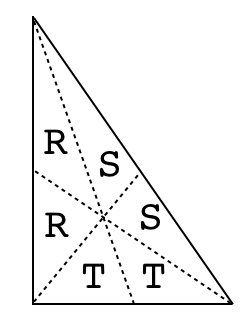
\includegraphics [scale=0.4] {centroid_tri.png} \end{center}

We draw lines from each vertex to the midpoint of the opposite side.  The three lines cross at a single point, the centroid.  (We looked at the proof of this in Ceva's Theorem).  It is easy to see that the areas of the small triangles with the same letter are equal.  For example, both $T$ have the same base (because we drew the median), and the same height.  For the same reason

\[ R + R + T = S + S + T \]
That is
\[ R = S = T \]
The extension to $T$ follows because the problem is symmetrical.  

Now consider the median shown in red in the figure below and the altitude drawn to it.

\begin{center} 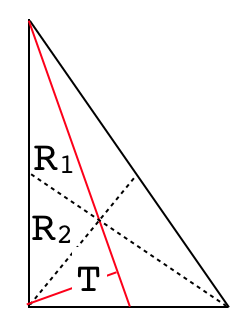
\includegraphics [scale=0.4] {centroid_tri2.png} \end{center}

Both the triangle labeled $T$ and the triangle formed from $R_1 + R_2$ have this as their height.  But the area of $R_1 + R_2$ is twice that of $T$.  Therefore the length of the base of $R_1 + R_2$ must be twice that for the triangle labeled $T$.  That is, the centroid lies at $2/3$ of the distance from the vertex to the opposing side.

Since we have a right triangle, then by similar triangles, the x-coordinate of the centroid is 
\[ \frac{2}{3} \frac{1}{2}= \frac{1}{3}\]
By symmetry, the y coordinate is at $1/3$ well.

The last part is the centroid of the half-circle.  According to Mathworld, this is

\[ \int y \ x \ dx \]
Since
\[ y = \sqrt{R^2-x^2} \]

\[ <y> \ = 2 \int_{0}^{R} y \ x \ dx \]
\[= 2 \int_{-R}^{R} \sqrt{R^2-x^2} \ x \ dx\]
Substitute $u=R^2-x^2$ and $du = -2x \ dx$
\[ = -\int \sqrt{u} \ du  = -\frac{2}{3} u^{3/2} \]
\[ = -\frac{2}{3} \ (R^2-x^2)^{3/2} \bigg |_0^R \]
\[ = \frac{2}{3} \ (R^2)^{3/2} \]
\[ = \frac{2}{3}R^3 \]
Since we integrated over the area, we must divide by $(1/2)\pi R^2$
\[ \bar{y} = \frac{<y>}{A} = \frac{2}{3}R^3 \ \frac{2}{\pi R^2} = \frac{4}{3} \frac{R}{\pi} \]



\end{document}  